\begin{frame}
\frametitle{About This Work...}

\emph{A Graph Model for False Negative Handling in Indoor RFID Tracking Data}.~\cite{baba2013graph} \\
A.I.~Baba, H.~Lu, T.B.~Pedersen, X.~Xie\\~\\

\begin{itemize}
  \item Published at \emph{SIGSPAITAL' 2013}.
  \item Focuses on handling \emph{false negatives} which occur when a moving object passes the detection range of an RFID reader but the reader fails to produce any readings.
  \item Proposes the transition probabilities that capture how likely objects move from one RFID reader to another.
\end{itemize}

\end{frame}

%------------------------------------------------

\begin{frame}
\frametitle{Motivation}

\begin{itemize}
  \item RFID emerges to be one of the key technologies to modernize object tracking and monitoring systems in indoor environments.
  \begin{sitemize}
    \item airport baggage tracking
  \end{sitemize}
  \item However, the unreliable nature of raw data captured by readers is a major factor hindering the development of various applications.
  \begin{sitemize}
    \item loss and error rate can be between 30-40\%.~\cite{floerkemeier2004issues}
    \item read events are frequently missed due to the detection ability of a reader, the quality of an RFID tag, and constraints of the environment.~\cite{derakhshan2007rfid}
  \end{sitemize}
  \item Critical to cleanse the RFID raw data, and provide clean data to high level applications to make correct interpretations and analysis of the physical world.
\end{itemize}

\end{frame}

%------------------------------------------------

\begin{frame}
\frametitle{False Negatives}

\begin{figure}[tb]
  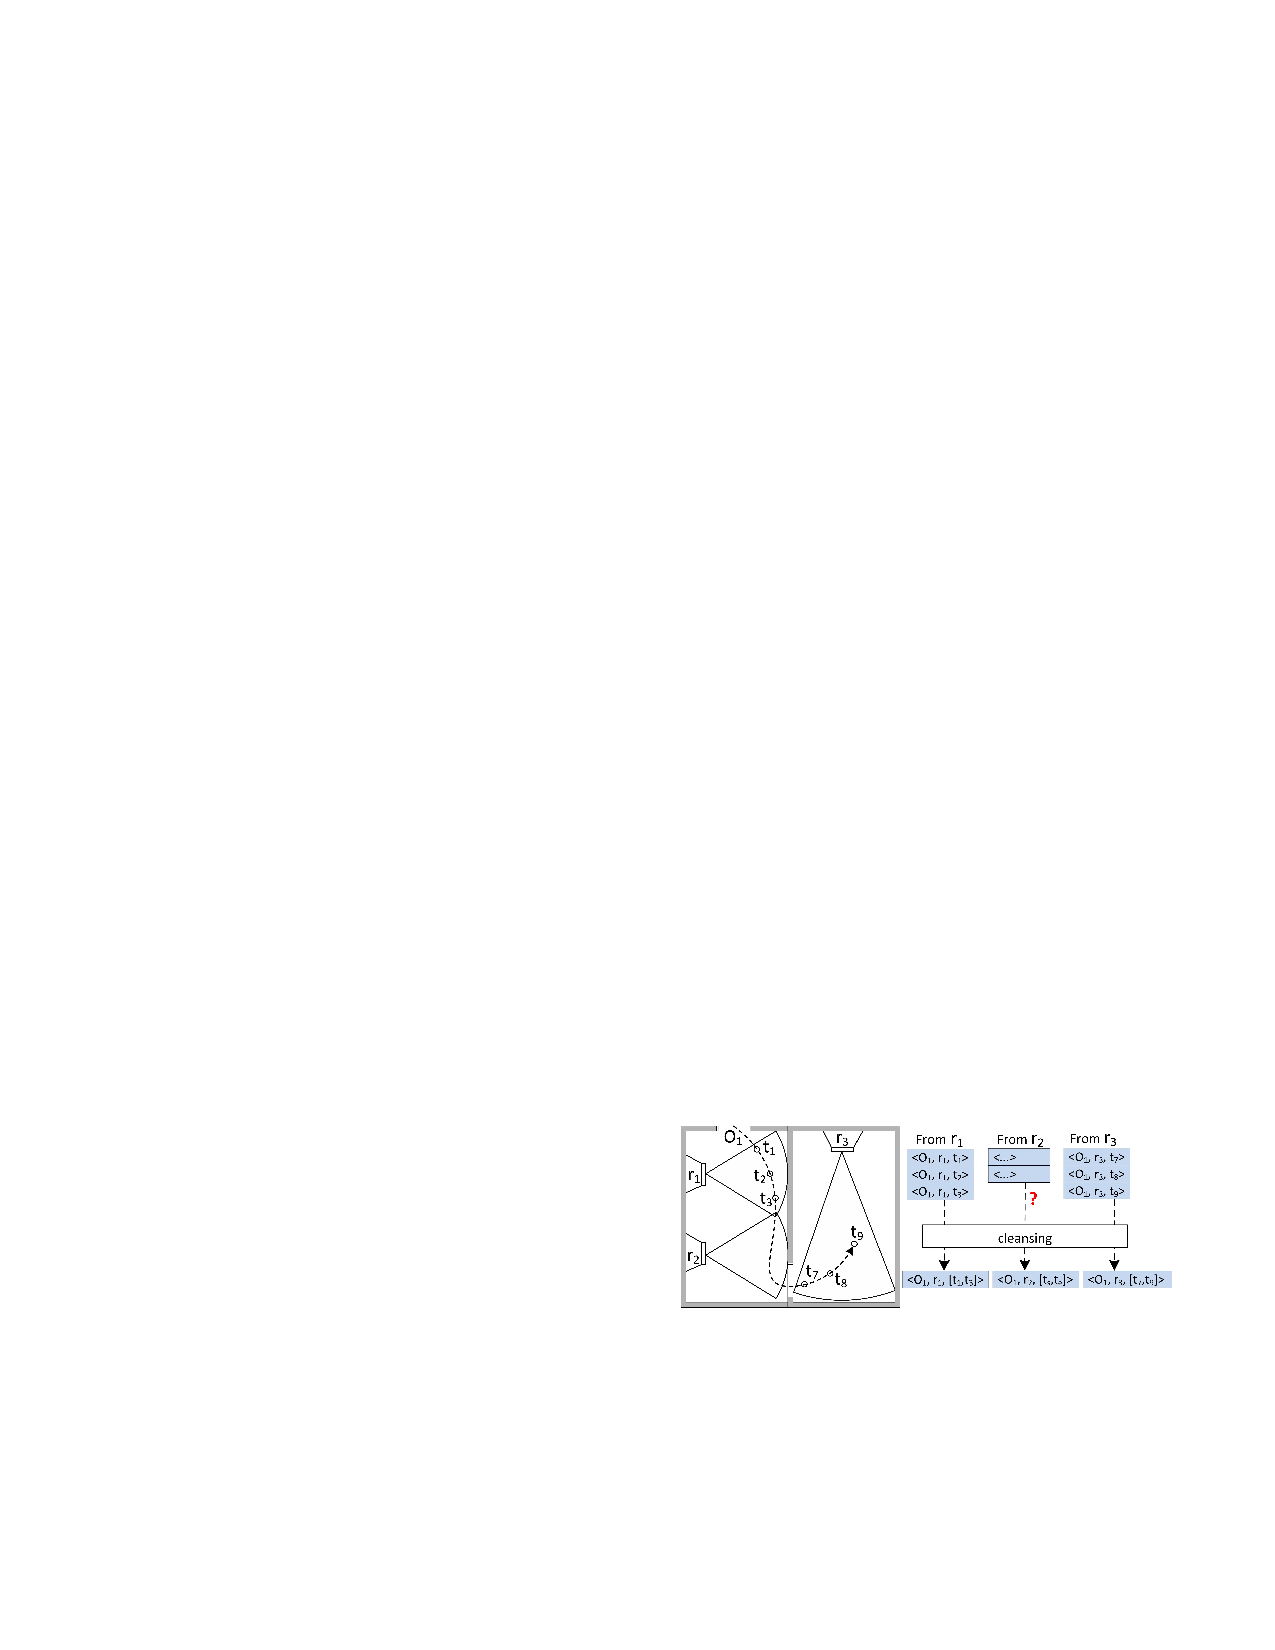
\includegraphics[width=0.8\columnwidth]{figures/3-3/3-3-1.pdf}
\end{figure}
\vspace{-10pt}
\begin{example}
  \ssize{
  two readers $r_1$ and $r_2$ in one hall and $r_3$ in another hall. Object $O_1$ enters the hall at time $t_1$ and is continuously tracked by $r_1$ until $t_3$. After that, $O_1$ is detected by $r_3$ at $t_7$ and $r_3$ keeps tracking $O_1$ until $t_9$. However, $O_1$ is not supposed to be detected by $r_3$ before it's detected by reader $r_2$ on its way, because to enter into the hall where $r_3$ is, $O_1$ must pass the detection range of $r_1$ and $r_2$ and cannot remain undetected for time interval $[t_3, t_7]$.
  }
\end{example}

\end{frame}

%------------------------------------------------

\begin{frame}
\frametitle{Aggregate Tracking Table (ATT)~\cite{baba2013spatiotemporal}}

\begin{itemize}

  \item All raw readings are ordered by their detection times and are aggregated into tracking records in \conceptbf{Aggregate Tracking Table}($ATT$).

  \item Each generated tracking record is in the format of $(deviceID, objectID, t_s, t_e, r_{Count})$.

  \item The meaning is that object identified by $objectID$ is detected by device identified by $deviceID$ during time interval $[t_s, t_e]$ for $r_{Count}$ times.
\end{itemize}

\end{frame}

%------------------------------------------------

\begin{frame}
\frametitle{Definitions}

\begin{definition}[False Negatives]
  Given a reader $r_i$ and a moving object $O$, if object $O$ goes through the detection range of reader $r_i$ during time interval $[t, t']$, but $r_i$ does not generate any reading about $O$'s presence during time interval $[t, t']$, a false negative occurs in the data.
\end{definition}

\begin{definition}[False Negatives Handling]
  Given an $ATT$, the false negative handling process detects false negatives and inserts recovered tracking records into the $ATT$.
\end{definition}

\end{frame}

%------------------------------------------------

\begin{frame}
\frametitle{Transition Probabilities} %Probabilistic Distance-Aware Graph Model



\end{frame}
